\section{LTE에 사용된 Modulation 기술}
이동통신에서는 무선 채널 상태가 매우 빠르고 크게 변화하기 때문에 최적의 통신 자원 할당을 위해 송신측이 수신측으로부터 채널 상태 정보를 수시, 정기적으로 보고 받아야 한다. LTE 네트워크에서 이동 단말이 채널의 품질을 측정하고, 이 정보를 주기적으로 기지국에 전달하는 상향링크 부채널/정보를 CQI(Channel Quality Indicator/Indication)이라고 한다. \\
각 단말에서 측정한 SINR 정보로 4 또는 5 비트의 CQI 정보를 표현하여 상향링크 제어 채널로 주기적(최대 5ms)마다 보고한다. 아래의 표는 LTE 네트워크의 SINR과 CQI mapping table의 예시이다. 기지국은 전달 받은 CQI code에 따라 modulation 방식과 code Rate을 바꾼다. 무선 채널 상태가 좋다면 높은 code rate와 modulation 방식을 사용하여 전송 속도를 증가시키고, 무선 채널 상태가 나쁘다면 낮은 code rate와 modulation 방식을 사용하여 전송 속도를 감소시킨다. \\
\vspace{-4mm}  
\begin{figure}[!h]\centering
	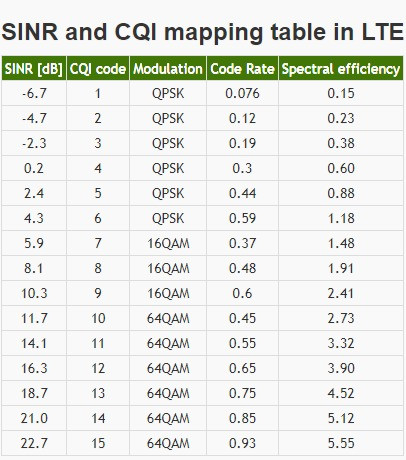
\includegraphics[width=.6\textwidth]{image/week11/2-1.png}
	\caption{\small SINR and CQI mapping table in LTE}
	\vspace{-10pt}
\end{figure}
Modulation(변조)란 이진수로 이루어진 디지털 정보를 저장, 전송하기 위해 전기적 신호로 변환하는 것이다. \\
일정한 형태의 반송파의 진폭, 주파수, 위상 등에 변화를 주어 디지털 정보를 담는다. 반송파 진폭에 변화를 주는 변조방식을 AM(Amplitude Modulation), 위상에 변화를 주는 변조방식을 PSK(Phase Shift Keying)라고 한다. 반송파 진폭과 위상 둘 모두 변화를 주는 변조방식을 QAM(Quadrature Amplitude Modulation)이라고 한다. \\
LTE 네트워크는 QPSK, 16QAM, 64QAM 혹은 그 이상의 modulation 방식을 사용한다. 각각은 4개(2bit), 16개(4bit), 64개(8bit)의 서로 다른 디지털 신호를 전송할 수 있다. \\
\vspace{-4mm}  
\begin{figure}[!h]\centering
	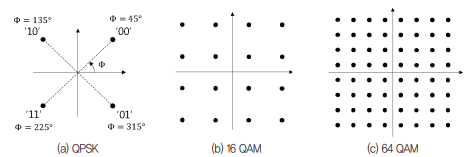
\includegraphics[width=.7\textwidth]{image/week11/2-2.png}
	\caption{\small Modulations, QPSK, 16QAM, 64QAM}
	\vspace{-10pt}
\end{figure}
\newpage